\documentclass[letter,11pt]{article}

\usepackage[spanish,es-nodecimaldot]{babel}
\usepackage[utf8]{inputenc}

\usepackage{lmodern}
\usepackage[T1]{fontenc}
\usepackage{textcomp}

\usepackage{framed}
\usepackage[svgnames]{xcolor}
\colorlet{shadecolor}{Gainsboro!50}

\usepackage[labelfont=bf]{caption}
\usepackage{graphicx}
\usepackage{pstricks}

\usepackage{anysize}
\marginsize{3cm}{2cm}{2cm}{3cm}

\usepackage{url}
\usepackage{siunitx}
\usepackage{amsmath}
\usepackage{array}
\usepackage{alltt}

\usepackage{caption}
\newcommand{\source}[1]{\vspace{-11pt} \caption*{\small{\textbf{Fuente:} {#1}}}}

\usepackage{fancyhdr}
\usepackage{lastpage}
\pagestyle{fancy}
\fancyhf{}
\fancyhead[LE,RO]{Laboratorio de Física Básica II}
\fancyfoot[CO,CE]{\thepage\ de \pageref{LastPage}}

\special{papersize=215.9mm,279.4mm}

\usepackage[
    pdfauthor={Carlos Eduardo Caballero Burgoa},%
    pdftitle={Laboratorio de Física Básica II},%
    pdfsubject={Constante elástica del resorte},%
    colorlinks,%
    citecolor=black,%
    filecolor=black,%
    linkcolor=black,%
    urlcolor=black,
    breaklinks]{hyperref}
\usepackage{breakurl}

\newcommand{\blankpage}{
\newpage
\thispagestyle{empty}
\mbox{}
\newpage
}

\renewcommand{\arraystretch}{1.2}

\title{Informe 2: Constante elástica del resorte}
\author{Carlos Eduardo Caballero Burgoa \\
    \small{\href{mailto:200201226@est.umss.edu}{200201226@est.umss.edu}}
}
\date{\today}

\begin{document}

\maketitle
\begin{center}
    \textbf{Grupo}: J2\\
    \textbf{Docente}: Ing. Milka Mónica Torrico Troche\\
    \textbf{Carrera}: Ing. Electromecánica
\end{center}

\begin{abstract}
    Este documento detalla el experimento realizado en simulador para calcular 
    la constante de proporcionalidad del resorte, a partir de la ley de
    \emph{Hooke}, para esto se realizó la medición de la elongación de un
    resorte a diferentes cantidades de masas disponibles; posteriormente se
    calculó la constante del resorte por medio del método de los mínimos
    cuadrados.
\end{abstract}

\section{Introducción}

\begin{figure}
\centering
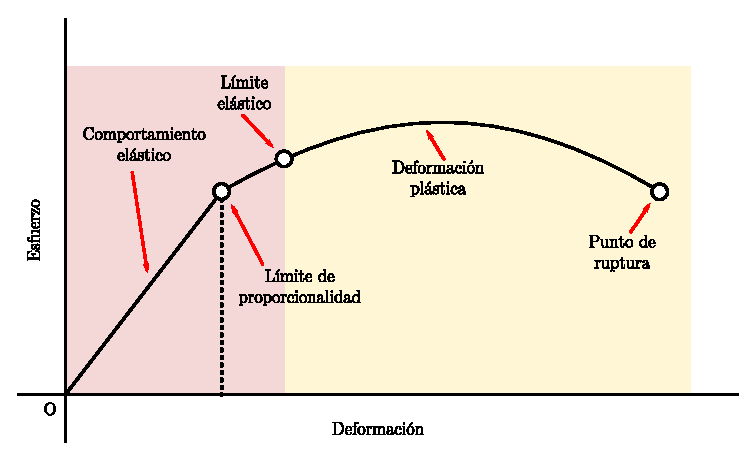
\includegraphics[width=0.40\textwidth]{resources/f1.eps}
\caption{Fuerza necesaria para estirar un resorte.}
\label{figura1}
\source{2013. Sears y Zemansky. Física Universitaria Volumen I. Pagina 188}
\end{figure}

Para mantener un resorte estirado una distancia $x$ más allá de su longitud sin
estirar, se debe aplicar una fuerza de igual magnitud en cada extremo como en la
\textbf{Figura \ref{figura1}}. Si el alargamiento $x$ no es excesivo, la fuerza
aplicada al extremo derecho tiene una componente $x$ directamente proporcional
a $x$, conocida como la ley de \emph{Hooke}:

\begin{equation}
    F_x = k x
\label{hooke}
\end{equation}
\vspace{0.25cm}

donde $k$ es una constante llamada \textbf{constante de fuerza} (o constante de
resorte). Las unidades de $k$ son de fuerza dividida entre distancia: $[N/m]$ en
el sistema internacional \cite{Sears y Zemansky}.

Para el experimento se verificará la ley de \emph{Hooke} citada anteriormente,
a partir de la toma de datos de elongación y fuerza, se graficaron los datos.
Finalmente se determinaron las constantes de los resortes usados.

\section{Método experimental}

Para la realización del experimento, se utilizará el simulador de resortes de
\emph{PHET}, ubicado en la dirección web:
\url{https://phet.colorado.edu/sims/html/masses-and-springs-basics/latest/masses-and-springs-basics_es.html},
este se muestra en la \textbf{Figura \ref{figura2}}.

\begin{figure}
\centering
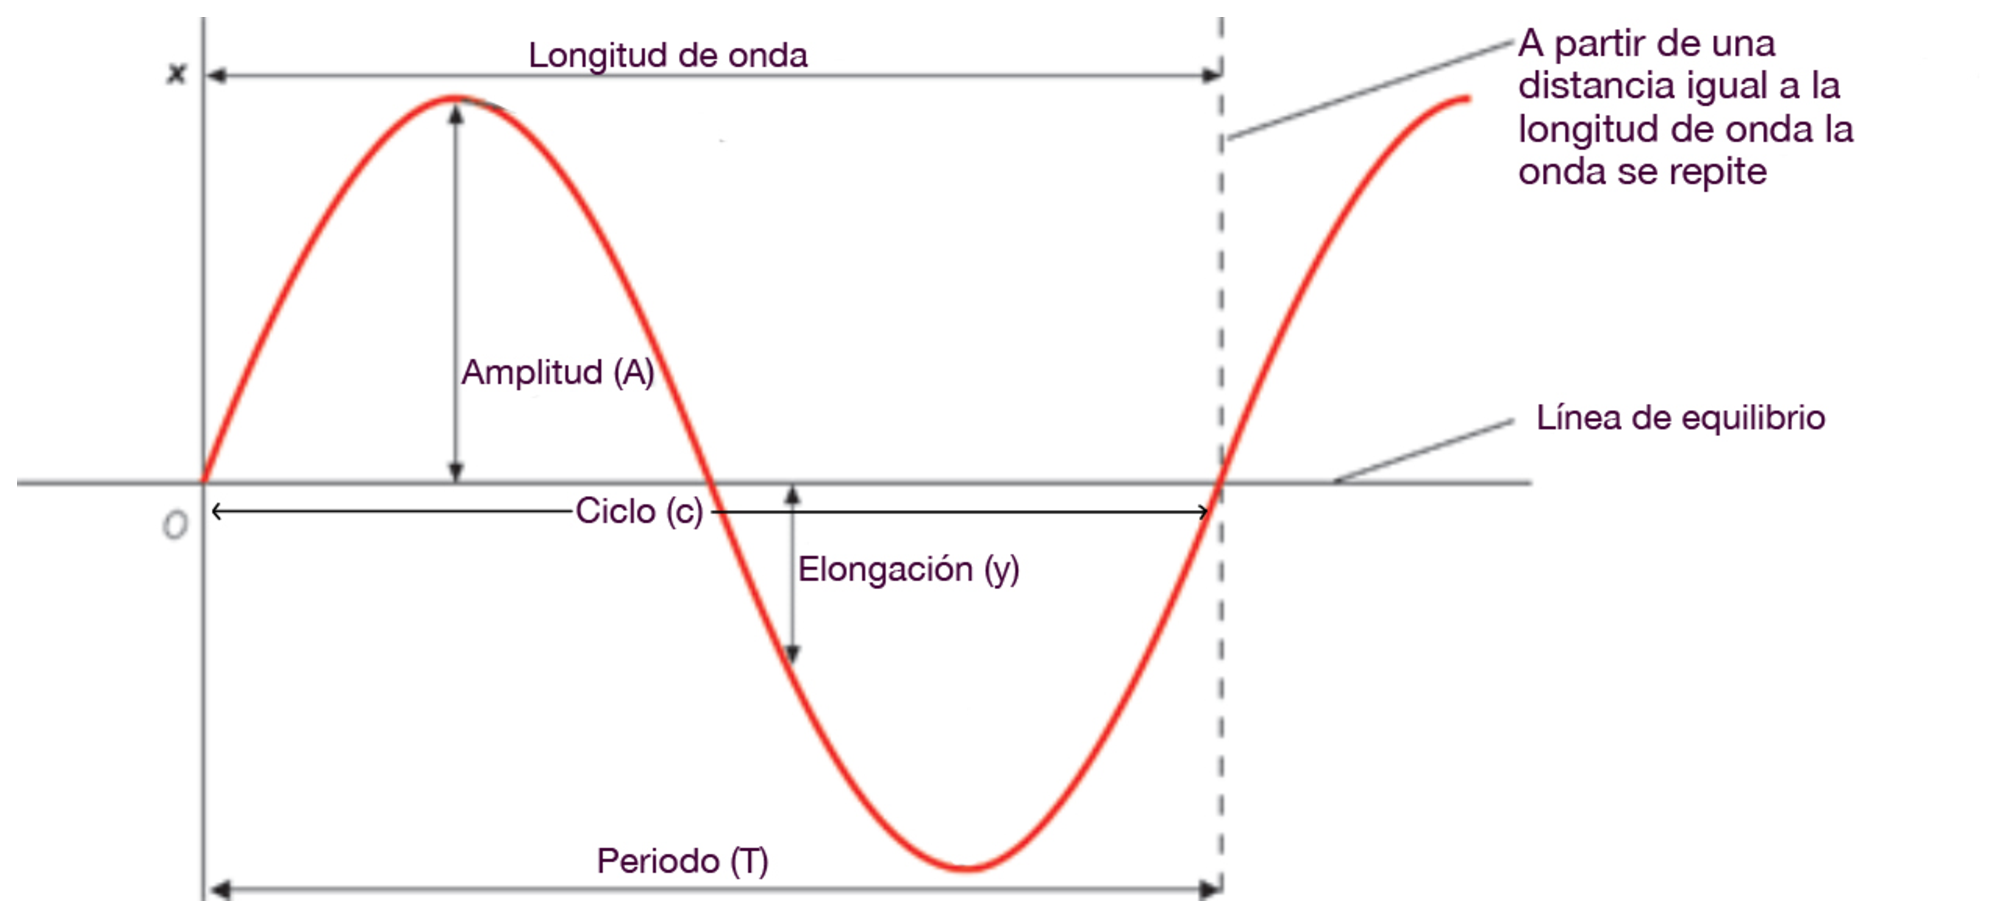
\includegraphics[width=0.90\textwidth]{resources/f2.eps}
\caption{Simulador de resortes.}
\label{figura2}
\source{Fotografía propia.}
\end{figure}

Para el simulador se escoge una fuerza del resorte, que se mantendrá constante
durante la medición, y se registrarán diferentes masas para medir su variación
de longitud.

Una vez medidos los datos para dos resortes con diferente fuerza del resorte,
se procederá a graficar la relación fuerza vs. longitud del resorte, y con la
ayuda del método de los mínimos cuadrados, se halla la relación funcional entre
las variables.

\vspace{0.35cm}
\textbf{Datos necesarios para el experimento:} \\

Aceleración de la gravedad local:
\begin{equation*}
    g = (9.78 \pm 0.02)[m/s^2]
\end{equation*}

Precisión de la regla:
\begin{equation*}
    P_l = 1 [cm]
\end{equation*}

Precisión de la balanza:
\begin{equation*}
    P_m = 1 [gr]
\end{equation*}

\section{Resultados}

\subsection{Resorte pequeño}
En el \textbf{cuadro \ref{cuadro1}}, pueden ver los valores tomados del 
experimento, tanto la masa como la longitud de la deformación resultante, para
una fuerza del resorte pequeña:

\begin{table}[!h]
\begin{center}
\begin{tabular}{|c|>{\centering}m{2.5cm}<{\centering}
                  |>{\centering}m{2.5cm}<{\centering}|}
\hline
$i$ & $m_i [g]$ & $x_i [cm]$ \tabularnewline \hline
 1 &   0 & 47 \tabularnewline \hline
 2 &  50 & 60 \tabularnewline \hline
 3 &  60 & 62 \tabularnewline \hline
 4 &  70 & 65 \tabularnewline \hline
 5 &  80 & 67 \tabularnewline \hline
 6 &  90 & 69 \tabularnewline \hline
 7 & 100 & 72 \tabularnewline \hline
 8 & 110 & 74 \tabularnewline \hline
 9 & 120 & 77 \tabularnewline \hline
10 & 130 & 79 \tabularnewline \hline
11 & 140 & 82 \tabularnewline \hline
12 & 150 & 84 \tabularnewline \hline
13 & 160 & 86 \tabularnewline \hline
14 & 170 & 89 \tabularnewline \hline
15 & 180 & 91 \tabularnewline \hline
16 & 190 & 94 \tabularnewline \hline
17 & 200 & 96 \tabularnewline \hline
18 & 210 & 99 \tabularnewline \hline
\end{tabular}
\caption{Mediciones de longitud en función de la masa provista.}
\label{cuadro1}
\source{Elaboración propia.}
\end{center}
\end{table}

A partir de los datos obtenidos se genera la gráfica de la
\textbf{Figura \ref{figura3}} de la fuerza y la longitud del resorte.

\begin{figure}
\centering
\includegraphics[width=0.80\textwidth]{resources/m1.eps}
\caption{Gráfica de longitud vs fuerza.}
\label{figura3}
\source{Elaboración propia.}
\end{figure}

Por tanto se realizo el ajuste de la curva, por el método de los mínimos
cuadrados, resultando:

\begin{equation*}
    a = (-0.0157 \pm 0.0074) [N]; 46.89 \%
\end{equation*}
\begin{equation*}
    b = (4.0031 \pm 0.0221) [N/m]; 0.55 \%
\end{equation*}
\begin{equation*}
    r = 0.9998
\end{equation*}

Sabiendo que el modelo de ajuste es:

\begin{equation*}
    F = a + b x
\end{equation*}
\vspace{0.25cm}

y despreciando el valor de $a$, obtenemos la siguiente relación funcional:

\begin{equation*}
    F \propto x
\end{equation*}
\vspace{0.25cm}

Por tanto, la constante elástica para el resorte pequeño del experimento es:

\begin{equation*}
    k = (4.0031 \pm 0.0221) [N/m]; 0.55 \%
\end{equation*}
\vspace{0.25cm}

\subsection{Resorte grande}
En el \textbf{cuadro \ref{cuadro2}}, pueden ver los valores tomados del 
experimento, tanto la masa como la longitud de la deformación resultante, para
una fuerza del resorte grande:

\begin{table}[!h]
\begin{center}
\begin{tabular}{|c|>{\centering}m{2.5cm}<{\centering}
                  |>{\centering}m{2.5cm}<{\centering}|}
\hline
$i$ & $m_i [g]$ & $x_i [cm]$ \tabularnewline \hline
 1 &   0 & 47 \tabularnewline \hline
 2 & 140 & 60 \tabularnewline \hline
 3 & 150 & 61 \tabularnewline \hline
 4 & 160 & 61 \tabularnewline \hline
 5 & 170 & 62 \tabularnewline \hline
 6 & 180 & 63 \tabularnewline \hline
 7 & 190 & 64 \tabularnewline \hline
 8 & 200 & 65 \tabularnewline \hline
 9 & 210 & 66 \tabularnewline \hline
10 & 220 & 67 \tabularnewline \hline
11 & 230 & 68 \tabularnewline \hline
12 & 240 & 69 \tabularnewline \hline
13 & 250 & 70 \tabularnewline \hline
14 & 260 & 70 \tabularnewline \hline
15 & 270 & 71 \tabularnewline \hline
16 & 280 & 72 \tabularnewline \hline
17 & 290 & 73 \tabularnewline \hline
18 & 300 & 74 \tabularnewline \hline
\end{tabular}
\caption{Mediciones de longitud en función de la masa provista.}
\label{cuadro2}
\source{Elaboración propia.}
\end{center}
\end{table}

A partir de los datos obtenidos se genera la gráfica de la
\textbf{Figura \ref{figura4}} de la fuerza y la longitud del resorte.

\begin{figure}
\centering
\includegraphics[width=0.80\textwidth]{resources/m2.eps}
\caption{Gráfica de longitud vs fuerza.}
\label{figura4}
\source{Elaboración propia.}
\end{figure}

Por tanto se realizo el ajuste de la curva, por el método de los mínimos
cuadrados, resultando:

\begin{equation*}
    a = (-0.0076 \pm 0.0253) [N]; 330.46 \%
\end{equation*}
\begin{equation*}
    b = (10.8946 \pm 0.1281) [N/m]; 1.18 \%
\end{equation*}
\begin{equation*}
    r = 0.9989
\end{equation*}

Sabiendo que el modelo de ajuste es:

\begin{equation*}
    F = a + b x
\end{equation*}
\vspace{0.25cm}

y despreciando el valor de $a$, obtenemos la siguiente relación funcional:

\begin{equation*}
    F \propto x
\end{equation*}
\vspace{0.25cm}

Por tanto, la constante elástica para el resorte grande del experimento es:

\begin{equation*}
    k = (10.8946 \pm 0.1281) [N/m]; 1.18 \%
\end{equation*}
\vspace{0.25cm}

\section{Discusión}

Puede notarse que en ambos resortes la variable $a$ es negativa, además que
el error de $b$ es pequeño, ambas son reflejo del uso de un simulador, ya que se
están tratando con resortes ideales.

\section{Conclusiones}

Se realizó la gráfica de longitud vs fuerza, donde es notoria la relación lineal
entre las variables.

Se realizó el ajuste de la curva por el método de mínimos cuadrados y se halló
la relación funcional entre estas dos variables, siendo está constante elástica
del resorte.

\begin{thebibliography}{99}

\bibitem{Sears y Zemansky} Sears y Zemansky (2013).\\
Física Universitaria. Volumen 1.\\
13va Edición.\\
Capitulo 11.

\end{thebibliography}

\newpage
\section*{Anexo: Cálculos adicionales}

\subsection{Resorte pequeño}
Conociendo $m_i$, $x_i$, y $g$, se detallan los valores de la fuerza calculada
($F$) y la longitud del estiramiento del resorte pequeño ($\Delta l$) en el
\textbf{cuadro \ref{cuadro3}}.

\begin{table}[!h]
\begin{center}
\begin{tabular}{|c|>{\centering}m{5.0cm}<{\centering}
                  |>{\centering}m{5.0cm}<{\centering}|}
\hline
$i$ & $F_i [N]$ & $\Delta x_i [m] $ \tabularnewline \hline
 1 & $(     0 \pm 0.0098)$ & $(     0 \pm 0.01)$ \tabularnewline \hline
 2 & $(0.4890 \pm 0.0098)$ & $(0.1300 \pm 0.01)$ \tabularnewline \hline
 3 & $(0.5868 \pm 0.0099)$ & $(0.1500 \pm 0.01)$ \tabularnewline \hline
 4 & $(0.6846 \pm 0.0099)$ & $(0.1800 \pm 0.01)$ \tabularnewline \hline
 5 & $(0.7824 \pm 0.0099)$ & $(0.2000 \pm 0.01)$ \tabularnewline \hline
 6 & $(0.8802 \pm 0.0099)$ & $(0.2200 \pm 0.01)$ \tabularnewline \hline
 7 & $(0.9780 \pm 0.0100)$ & $(0.2500 \pm 0.01)$ \tabularnewline \hline
 8 & $(1.0758 \pm 0.0100)$ & $(0.2700 \pm 0.01)$ \tabularnewline \hline
 9 & $(1.1736 \pm 0.0101)$ & $(0.3000 \pm 0.01)$ \tabularnewline \hline
10 & $(1.2714 \pm 0.0101)$ & $(0.3200 \pm 0.01)$ \tabularnewline \hline
11 & $(1.3692 \pm 0.0102)$ & $(0.3500 \pm 0.01)$ \tabularnewline \hline
12 & $(1.4670 \pm 0.0102)$ & $(0.3700 \pm 0.01)$ \tabularnewline \hline
13 & $(1.5648 \pm 0.0103)$ & $(0.3900 \pm 0.01)$ \tabularnewline \hline
14 & $(1.6626 \pm 0.0104)$ & $(0.4200 \pm 0.01)$ \tabularnewline \hline
15 & $(1.7604 \pm 0.0104)$ & $(0.4400 \pm 0.01)$ \tabularnewline \hline
16 & $(1.8582 \pm 0.0105)$ & $(0.4700 \pm 0.01)$ \tabularnewline \hline
17 & $(1.9560 \pm 0.0106)$ & $(0.4900 \pm 0.01)$ \tabularnewline \hline
18 & $(2.0538 \pm 0.0106)$ & $(0.5200 \pm 0.01)$ \tabularnewline \hline
\end{tabular}
\caption{Calculo de la fuerza y la longitud.}
\label{cuadro3}
\source{Elaboración propia.}
\end{center}
\end{table}

\subsection{Resorte grande}
Conociendo $m_i$, $x_i$, y $g$, se detallan los valores de la fuerza calculada
($F$) y la longitud del estiramiento del resorte grande ($\Delta l$) en el
\textbf{cuadro \ref{cuadro4}}.

\begin{table}[!h]
\begin{center}
\begin{tabular}{|c|>{\centering}m{5.0cm}<{\centering}
                  |>{\centering}m{5.0cm}<{\centering}|}
\hline
$i$ & $F_i [N]$ & $\Delta x_i [m] $ \tabularnewline \hline
 1 & $(     0 \pm 0.0098)$ & $(     0 \pm 0.01)$ \tabularnewline \hline
 2 & $(1.3692 \pm 0.0102)$ & $(0.1300 \pm 0.01)$ \tabularnewline \hline
 3 & $(1.4670 \pm 0.0102)$ & $(0.1400 \pm 0.01)$ \tabularnewline \hline
 4 & $(1.5648 \pm 0.0103)$ & $(0.1400 \pm 0.01)$ \tabularnewline \hline
 5 & $(1.6626 \pm 0.0104)$ & $(0.1500 \pm 0.01)$ \tabularnewline \hline
 6 & $(1.7604 \pm 0.0104)$ & $(0.1600 \pm 0.01)$ \tabularnewline \hline
 7 & $(1.8582 \pm 0.0105)$ & $(0.1700 \pm 0.01)$ \tabularnewline \hline
 8 & $(1.9560 \pm 0.0106)$ & $(0.1800 \pm 0.01)$ \tabularnewline \hline
 9 & $(2.0538 \pm 0.0106)$ & $(0.1900 \pm 0.01)$ \tabularnewline \hline
10 & $(2.1516 \pm 0.0107)$ & $(0.2000 \pm 0.01)$ \tabularnewline \hline
11 & $(2.2494 \pm 0.0108)$ & $(0.2100 \pm 0.01)$ \tabularnewline \hline
12 & $(2.3472 \pm 0.0109)$ & $(0.2200 \pm 0.01)$ \tabularnewline \hline
13 & $(2.4450 \pm 0.0110)$ & $(0.2300 \pm 0.01)$ \tabularnewline \hline
14 & $(2.5428 \pm 0.0111)$ & $(0.2300 \pm 0.01)$ \tabularnewline \hline
15 & $(2.6406 \pm 0.0112)$ & $(0.2400 \pm 0.01)$ \tabularnewline \hline
16 & $(2.7384 \pm 0.0113)$ & $(0.2500 \pm 0.01)$ \tabularnewline \hline
17 & $(2.8362 \pm 0.0114)$ & $(0.2600 \pm 0.01)$ \tabularnewline \hline
18 & $(2.9340 \pm 0.0115)$ & $(0.2700 \pm 0.01)$ \tabularnewline \hline
\end{tabular}
\caption{Calculo de la fuerza y la longitud.}
\label{cuadro4}
\source{Elaboración propia.}
\end{center}
\end{table}

\end{document}

